\documentclass[a4paper,12pt, oneside]{book}

%\usepackage{fullpage}
\usepackage[italian]{babel}
\usepackage[utf8]{inputenc}
\usepackage{amssymb}
\usepackage{amsthm}
\usepackage{graphics}
\usepackage{amsfonts}
\usepackage{listings}
\usepackage{amsmath}
\usepackage{amstext}
\usepackage{engrec}
\usepackage{rotating}
\usepackage[safe,extra]{tipa}
\usepackage{showkeys}
\usepackage{multirow}
\usepackage{hyperref}
\usepackage{microtype}
\usepackage{enumerate}
\usepackage{braket}
\usepackage{marginnote}
\usepackage{pgfplots}
\usepackage{cancel}
\usepackage{polynom}
\usepackage{booktabs}
\usepackage{enumitem}
\usepackage{framed}
\usepackage{pdfpages}
\usepackage{pgfplots}
\usepackage[cache=false]{minted}

\usepackage{tikz}\usetikzlibrary{er}\tikzset{multi  attribute /.style={attribute ,double  distance =1.5pt}}\tikzset{derived  attribute /.style={attribute ,dashed}}\tikzset{total /.style={double  distance =1.5pt}}\tikzset{every  entity /.style={draw=orange , fill=orange!20}}\tikzset{every  attribute /.style={draw=MediumPurple1, fill=MediumPurple1!20}}\tikzset{every  relationship /.style={draw=Chartreuse2, fill=Chartreuse2!20}}\newcommand{\key}[1]{\underline{#1}}

\usepackage{fancyhdr}
\pagestyle{fancy}
\fancyhead[LE,RO]{\slshape \rightmark}
\fancyhead[LO,RE]{\slshape \leftmark}
\fancyfoot[C]{\thepage}



\title{Basi di Dati}
\author{UniShare\\\\Davide Cozzi\\\href{https://t.me/dlcgold}{@dlcgold}\\\\Gabriele De Rosa\\\href{https://t.me/derogab}{@derogab} \\\\Federica Di Lauro\\\href{https://t.me/f_dila}{@f\textunderscore dila}}
\date{}

\pgfplotsset{compat=1.13}
\begin{document}
\maketitle

\definecolor{shadecolor}{gray}{0.80}

\newtheorem{teorema}{Teorema}
\newtheorem{definizione}{Definizione}
\newtheorem{esempio}{Esempio}
\newtheorem{corollario}{Corollario}
\newtheorem{lemma}{Lemma}
\newtheorem{osservazione}{Osservazione}
\newtheorem{nota}{Nota}
\newtheorem{esercizio}{Esercizio}
\tableofcontents
\renewcommand{\chaptermark}[1]{%
\markboth{\chaptername
\ \thechapter.\ #1}{}}
\renewcommand{\sectionmark}[1]{\markright{\thesection.\ #1}}
\chapter{Introduzione}
\textbf{Questi appunti sono presi a ldurante le esercitazioni in laboratorio. Per quanto sia stata fatta una revisione è altamente probabile (praticamente certo) che possano contenere errori, sia di stampa che di vero e proprio contenuto. Per eventuali proposte di correzione effettuare una pull request. Link: } \url{https://github.com/dlcgold/Appunti}.\\
\textbf{Grazie mille e buono studio!}
\chapter{E-R}
Il corso si divide in 7 parti:
\begin{enumerate}
\item introduzione generale
\item metodologie e modelli per il progetto delle basi di dati
\item progettazione concettuale
\item modello razionale
\item progettazione logica
\item linguaggio SQL
\item algebra relazionale
\end{enumerate}
Le \textbf{informazioni} fanno parte delle risorse di un'azienda. Una \textbf{base di dati} \textit{è un insieme organizzato di dati utilizzato per il supporto allo svolgimento di attività.} L'\textbf{informatica} è la \textit{scienza del trattamento relazionale, specialmente per mezzo di macchine automatiche, dell'informazione, considerata come supporto alla conoscenza umana e all'informazione}. Un \textbf{sistema informativo} è \textit{un componente di un'organizzazione che gestisce le informazioni d'interesse}. Si divide in:
\begin{itemize}
\item acquisizione e memorizzazione
\item aggiornamento
\item interrogazione
\item elaborazione
\end{itemize}
Un sistema informativo è una porzione automatizzata del sistema informatico. Un sistema informatico gestisce il sistema informativo in modo automatizzato, ne garantisce la memorizzazione, l'aggiornamento dei dati per riflettere le loro variazioni, l'accessibilità dei dati. Un sistema informatico può essere distribuito sul territorio. Le informazioni vengono gestite in vari modi, mediante idee formali, con il linguaggio naturale, graficamente con schemi e con numeri o codici. Anche il mezzo può variare dalla carta ai dispositivi elettronici. Pian piano si è arrivato ad avere una codifica standard per l'informazione, a fini organizzativi. Le informazioni nei sistemi informatici sono rappresentate in modo essenziale mediante i \textbf{dati}, questa è la \textit{sintassi}. La \textit{semantica} invece si ottiene con le intestazioni delle tabelle. I dati sono una risorsa strategica perché sono stabili nel tempo. Solitamente i dati sono immutati durante una migrazione tra un sistema e un altro. Un \textbf{Data Base} è una collezione di dati usati per rappresentare un'informazione di interesse di un sistema informativo. Un \textbf{DBMS} è un software che gestisce un database. Un base di dati è anche un insieme di archivi in cui ogni dato è rappresentato logicamente una e una sola volta è può essere usato da un insieme di applicazioni e da più utenti su vari criteri di riservatezza. Si hanno le seguenti caratteristiche:
\begin{itemize}
\item i dati sono molti
\item i dati hanno un formato definito
\item i dati sono permanenti
\item i dati sono raggruppati per insiemi omogenei di dati
\item esistono relazioni specifiche tra gli insiemi di dati
\item la ridondanza minima è controllata ed è assicurata la consistenza delle informazioni
\item i dati sono disponibili per utenze diverse  e concorrenti
\item i dati sono controllati e  protetti da
malfunzionamenti hardware e software
\item i dati sono indipendenti dal programma
\end{itemize}
Si hanno tre fasi di creazione di una tabella:
\begin{enumerate}
\item definizione
\item creazione e popolazione
\item manipolazione
\end{enumerate}
Si garantiscono:
\begin{itemize}
\item privatezza
\item affidabilità
\item efficienza
\item efficacia
\end{itemize}
Un organizzazione è divisa in vari settori e ogni settore ha un suo sottosistema informativo (non necessariamente disgiunto). Le basi dati solitamente sono condivise. Una base di dati gestisce i meccanismi di autorizzazione e ha un controllo della concorrenza, oltre ad essere una risorsa integrata e condivisa. Una base di dati deve essere conservata a lungo termine e si ha una gestione delle \textbf{transazioni}. Una \textbf{transazione} \textit{è un insieme di operazioni da considerare indivisibile, "atomico", corretto anche in presenza di concorrenza e con effetti definitivi}. La sequenza di operazioni sulla base di dati deve essere eseguita nella sua interezza (sono quindi atomiche) e l'effetto di transazioni concorrenti deve essere coerente. La conclusione positiva di una transazione corrisponde ad un impegno, \textit{commit}, a mantenere traccia del risultato in modo definitivo, anche in presenza di guasti e di esecuzione concorrente.\\
I DBMS devono essere efficienti, utilizzando al meglio memoria e tempo. Devono anche essere efficaci e produttivi. \\
Si hanno delle caratteristiche nell'apporoccio alla base dati:
\begin{itemize}
\item natura autodescrittiva di un sistema di basi
di dati: il sistema di basi di dati memorizza i dati e
anche una descrizione completa della sua
struttura (catalogo) queste informazioni sono
chiamate metadati. Questo consente al DBMS di
lavorare con qualsiasi applicazione
\item separazione tra programmi e dati: chiamata
indipendenza tra programmi e dati. E’ possibile
cambiare la struttura dati senza cambiare i
programmi
\item astrazione dei dati: Si usa un modello dati
per nascondere dettagli e presentare all'utente
una vista concettuale del database
\item supporto di viste multiple dei dati: Ogni
utente può usare una vista (view) differente del
database, contenente solo i dati di interesse per
quell'utente
\item condivisione dei dati e gestione delle
transazioni con utenti multipli. Permette a più
utenti concorrenti di accedere contemporaneamente
al database. Il controllo della concorrenza
garantisce che più utenti impegnati ad aggiornare gli
stessi dati lo facciano in maniera controllata: il
risultato degli aggiornamenti è corretto
\end{itemize}
I DBMS estendono le funzionalità dei file
system, fornendo più servizi ed in maniera integrata.
\\In ogni base di dati si ha:
\begin{itemize}
\item lo \textbf{schema}, sostanzialmente invariante nel
tempo, che ne descrive la struttura, il
significato (aspetto intensionale, ovvero la descrizione
"astratta" delle proprietà, ed è invariante
nel tempo).
\item l'\textbf{istanza}, i valori attuali, che possono
cambiare anche molto rapidamente (aspetto estensionale "concreto", che varia nel
tempo al variare della situazione di ciò
che stiamo descrivendo)
\end{itemize}
Si hanno due tipi di modelli:
\begin{itemize}
\item \textbf{modelli logici}, adottati nei DBMS esistenti per l'organizzazione dei dati, utilizzati dai programmi e indipendenti dalle strutture fisiche
\item \textbf{modelli concettuali} che permettono di rappresentare i dati in modo indipendente da ogni sistema, che cercano di descrivere i concetti del mondo reali e sono usati delle fasi preliminari di progettazione. Il più diffuso è il modello \textbf{Entity-Relationship}
\end{itemize}
ecco l'architettura di un DBMS:
$$utente$$
$$\downarrow$$
$$schema\,\,\,logico$$
$$\downarrow$$
$$schema\,\,\,interno$$
$$\downarrow$$
$$database$$
Si hanno 2 schemi:
\begin{enumerate}
\item \textbf{schema logico:} descrizione della base
di dati nel modello logico (ad esempio,
la struttura della tabella)
\item \textbf{schema interno (o fisico):}
rappresentazione dello schema logico
per mezzo di strutture memorizzazione
(file; ad esempio, record con puntatori,
ordinati in un certo modo)
\end{enumerate}
Il livello logico è indipendente da quello
fisico infatti una tabella è utilizzata nello stesso modo
qualunque sia la sua realizzazione fisica
(che può anche cambiare nel tempo). \textbf{Noi tratteremo solo il livello logico}.
%immagine architettura standard
Ecco i tre schemi dell'architettura ANSI/SPARC:
\begin{enumerate}
\item \textbf{schema logico: }descrizione dell'intera base di
dati nel modello logico “principale” del DBMS
\item \textbf{schema fisico: }rappresentazione dello
schema logico per mezzo di strutture fisiche
di memorizzazione
\item\textbf{ schema esterno:} descrizione di parte della
base di dati in un modello logico (“viste”
parziali, derivate, anche in modelli diversi)
\end{enumerate}
L'accesso ai dati avviene solo mediante il livello esterno (che a volte coincide con quello logico) e si hanno 2 forme di indipendenza:
\begin{enumerate}
\item \textbf{indipendenza fisica} 
\item \textbf{indipendenza logica}
\end{enumerate}
Il livello logico e quello esterno sono
indipendenti da quello fisico.\\
Un linguaggio interattivo per gestire una base dati è SQL, che funziona tramite \textbf{query}. Si hanno linguaggi per la definizione di dati, i DLL, \textit{Data Definition Languages}, e linguaggi di manipolazione dei dati, DML, \textit{Data Manipulation Languages}. I primi definiscono e i secondi interrogano e aggiornano. SQL può svolgere le operazioni di entrambi.\\
SI hanno due tipi di utenti:
\begin{enumerate}
\item \textbf{utenti finali (terminalisti):} eseguono applicazioni
predefinite (transazioni)
\item \textbf{utenti casuali:} eseguono operazioni non previste
a priori, usando linguaggi interattivi
\end{enumerate}
inoltre si hanno:
\begin{itemize}
\item progettisti e realizzatori di DBMS
\item progettisti della base di dati e
amministratori della base di dati (DBA), persona o gruppo di persone responsabile del controllo centralizzato
e della gestione del sistema, delle
prestazioni, dell'affidabilità, delle
autorizzazioni. Le funzioni del DBA includono quelle di
progettazione, anche se in progetti
complessi ci possono essere distinzioni
\item progettisti e programmatori di applicazioni
\end{itemize}
\begin{center}
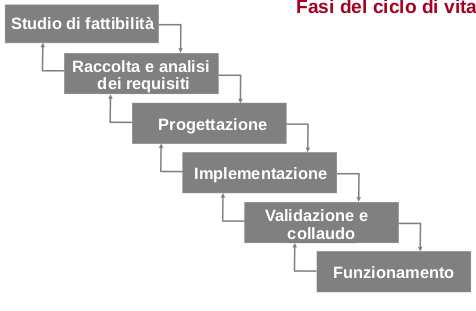
\includegraphics[scale=0.8]{img/bas.png}
\end{center}
Si hanno le seguenti fasi del ciclo di vita:
\begin{itemize}
\item \textbf{studio di fattibilità}, definizione di costi, priorità e competenze per un progetto
\item\textbf{raccolta e analisi dei requisiti}, ovvero lo studio delle proprietà del sistema
\item \textbf{progettazione} di dati e funzioni
\item \textbf{implementazione}
\item \textbf{validazione e collaudo},che comprendono anche test da parte del cliente
\item \textbf{funzionamento}, ovvero lo stadio finale dove il sistema diventa effettivamente operativo
\end{itemize}
ogni fase può tornare a quella precedente in caso di problemi. Prima di implementare una base di dati bisogna avere delle specifiche ben definite. \\
Si ha quindi un ciclo di vita con \textbf{modello a spirale}, in quanto ogni software deve avere delle releases, e per ognuna si ripete il ciclo di vita.\\
In questo processo a rimanere stabili sono prettamente i \textbf{dati}. Prima si progetta la base dati, con una \textbf{metodologia di progetto}, e poi l'applicazione:
\begin{center}
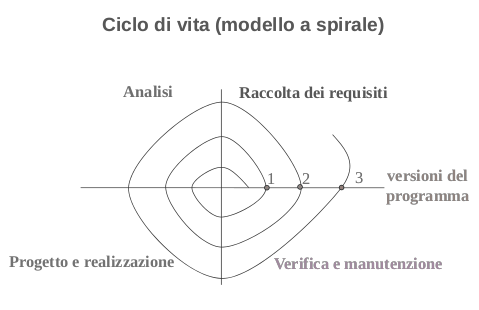
\includegraphics[scale=2.8]{img/bas2.png}
\end{center}
1
Una \textbf{metodologia} è un'articolazione in fasi di guida ad un'attività di progettazione. Per una base dati serve una metodologia che:
\begin{itemize}
\item suddivida la progettazione in fasi indipendenti
\item fornisca strategie e criteri di scelta in caso di alternative
\item fornisca modelli di riferimento (i linguaggi)
\item garantisca generalità rispetto al problema
\item garantisca qualità e facilità d'uso
\end{itemize}
Si separa il cosa rappresentare e il come farlo.\\
Si parte dalla progettazione concettuale, si passa a quella logica e si finisce con quella fisica.
\begin{center}
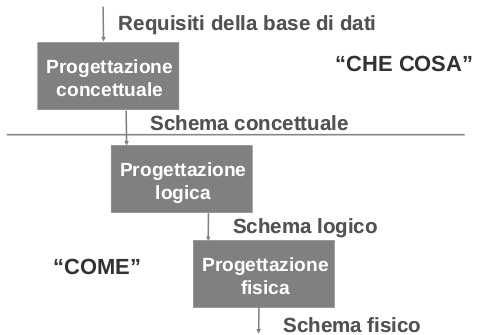
\includegraphics[scale=2.5]{img/bas3.png}
\end{center}
\begin{center}
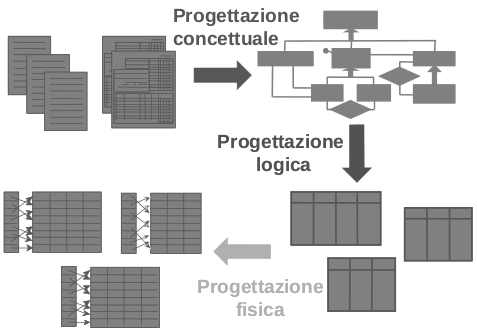
\includegraphics[scale=2.5]{img/bas4.png}
\end{center}
Ognuna di queste 3 fasi si basa su un modello che permette di generare una rappresentazione formale, uno schema, delle basi di dati ad un dato livello di astrazione: schema concettuale, schema logico e schema fisico. 
\begin{itemize}
\item la \textbf{progettazione concettuale} consiste nel tradurre i requisiti del sistema informatico in una descrizione formale, integrata e indipendente dalle scelte
implementative (DBMS, SW e HW)
\item la \textbf{progettazione concettuale} consiste nella traduzione dello schema con concettuale nel modello dei dati del DBMS Il risultato è uno schema logico, espresso nel DDL
del DBMS. In questa fase si considerano anche aspetti legati ai vincoli ed all'efficienza. Si hanno due sotto-fasi:
\begin{itemize}
\item ristrutturazione dello schema concettuale
\item traduzione verso il modello logico
\end{itemize}
\item la \textbf{progettazione fisica} completa lo
schema logico ottenuto con le
specifiche proprie dell'hw/sw scelto.
Il risultato è lo schema fisico che descrive le strutture
di memorizzazione ed accesso ai dati
\end{itemize}
si ha quindi:
\begin{center}
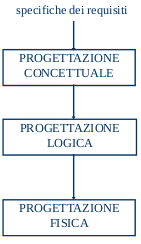
\includegraphics[scale=0.7]{img/bas5.png}
\end{center}
Nel nostro caso si ha che il modello E-R è lo schema concettuale e lo schema logico è dato dal modello razionale.\\
Si hanno dei vantaggi con la progettazione concettuale, prevale infatti l'aspetto intensionale indipendente dalla tecnologia ed è una rappresentazione grafica. È utile per la documentazione.\\
In uno schema E-R abbiamo le entità, in costrutti,  rappresentati da rettangoli e le relazioni da rombi, con indicata l'arità (la cardinalità) (come in un UML). Esistono varie versioni del modello Entità-Relazione \textit{ER}.
si hanno i seguenti costrutti:
\begin{itemize}
\item entità
\item relazione
\item attributo semplice
\item attributo composto
\item cardinalità
\item cardinalità di un attributo
\item identificatore interno
\item identificatore esterno
\item generalizzazione
\item sottoinsieme
\end{itemize}
così rappresentati:
\begin{center}
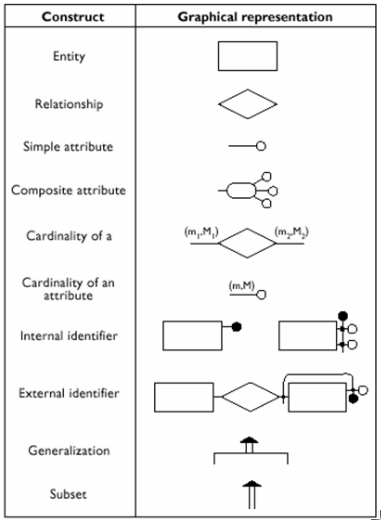
\includegraphics[scale=0.8]{img/bas6.png}
\end{center}
Un entità è una classe di oggetti dell'applicazione di interesse con proprietà comune con esistenza "autonoma" e della quale si vogliono specificare fatti specifici. Ogni entità ha un nome che la identifica univocamente, con le seguenti specifiche:
\begin{itemize}
\item si hanno nomi espressivi
\item si usa il singolare
\end{itemize}
Un'occorrenza, o istanza, di un'entità, è un oggetto della classe che l'entità rappresenta, ma noi rappresentiamo le entità dello schema concettuale non le singole istanze. Si parla di \textit{ conoscenza astratta} se si parla di entità e di \textit{conoscenza concreta} se si parla di un'istanza di un'entità. Ovviamente un elemento della classe ha degli attributi, rappresentati da dei pallini collegati alla classe. Un attributo ha un dominio che però non viene rappresentato nell'E-R ma nella documentazione. Entità e attributi funzionano con determinate regole, un attributo è una funzione:
\begin{itemize}
\item un enità non può avere valori diversi della stesso attributo
\item due entità possono avere lo stesso valore di un attributo
\item bisogna sempre specificare il valore di un attributo, si ha una funzione totale
\end{itemize}
Si ha che gli \textbf{attributi composti} si ottengono raggruppando attributi di una
medesima entità o relazione che presentano
affinità nel loro significato o uso (per esempio per un indirizzo si ha via, comune, cap etc...). Nessuno impone un tipo per un certo attributo, possono essere anche complessi di cui però non ci interessano le informazioni che lo rappresentano (per esempio una foto può essere un attributo, ma se ho bisogno, per esempio, dell'autore della foto, non sarà più un attributo ma un'altra entità). \\
Un'associazione, o relazione, è un fatto che descrive un'azione o una situazione e che stabilisce legami logici tra
istanze di entità (associa, mette in relazione)
nella realtà che stiamo considerando. Si possono avere legami tra più entità e il numero di entità coinvolte in una relazione ne determina il \textbf{grado}. Valgono le stesse regole delle entità per dare un nome alle relazioni (nomi espressivi e al singolare) ma se ne aggiunge una: si usano sostantivi e non verbi. \\
Un'\textbf{istanza di associazione} è un a combinazione o aggregazione di istanze di entità che prendono parte all'associazione (per esempio "prof. Schettini" è istanza di associazione per l'entità docente). Dalla semantica delle relazioni segue immediatamente che non possono esistere due istanze della stessa relazione che coinvolgono le stesse istanze di entità.\\
\textbf{Due entità possono essere coinvolte in più relazioni}
\\
Le relazioni possono avere attributi, con valori specificati in un certo dominio. Un attributo di una relazione tra più entità modella una proprietà del legame tra tutte le entità rappresentato dalla relazione. Gli attributi delle relazioni si rappresentano come quelli di entità.

\newpage
\textit{Descrivere lo schema concettuale della seguente
realtà:
I docenti hanno un codice fiscale ed una età. I
docenti operano nei corsi di laurea (si dice che
afferiscono ai corsi di laurea). Interessa la data di
afferenza dei docenti ai corsi di laurea. I corsi di
laurea hanno un codice ed un nome, ed
appartengono alle facoltà. Ogni facoltà ha un nome}
\begin{center}
\begin{tikzpicture}[node  distance =7em]
\node[entity] (docente) {docente};
\node[attribute] (età) [above left of =  docente] {età} edge (docente);
\node[attribute] (codice) [above of = docente] {codice fiscale} edge (docente);
\node[relationship] (operatore) [right of = docente] {operatore} edge (docente);
\node[attribute] (data) [below of = operatore ] {data} edge (operatore);
\node [entity] (laurea) [right of = operatore] {laurea} edge (operatore);
\node[attribute] (cod) [above of =  laurea] {nome} edge (laurea);
\node[attribute] (nome) [above right of = laurea] {codice} edge (laurea);
\node[relationship] (appartenenza) [below of = laurea] {appartenenza} edge (laurea);
\node [entity] (facoltà) [below of = appartenenza] {facoltà} edge (appartenenza);
\node[attribute] (nomee) [below of = facoltà] {nome} edge (facoltà);
\end{tikzpicture}
\end{center}
\newpage
Una associazione può coinvolgere “due o più volte”
la stessa entità. Si ha un'\textit{associazione ricorsiva o ad anello}:
\begin{center}
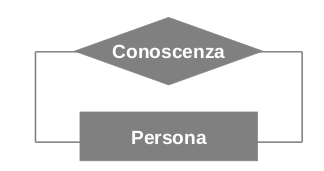
\includegraphics[scale=2.5]{img/bas7.png}
\end{center}
Un'associazione ad anello può essere o meno:
\begin{itemize}
\item \textbf{simmetrica:} $(a,b)\in A\to (b,a)\in A$
\item \textbf{riflessiva:} $(a,a)\in A$
\item \textbf{transitiva:} $(a,b)\in A,\,(b,c)\in A \to (a,c)\in A$
\end{itemize}
Nel caso sopra l'associazione conoscenza è simmetrica,
irriflessiva e intransitiva.\\
Nelle relazioni dove una stessa entità è coinvolta più volte è necessario aggiungere la specifica dei \textbf{ruoli}, come nell'esempio:
\begin{center}
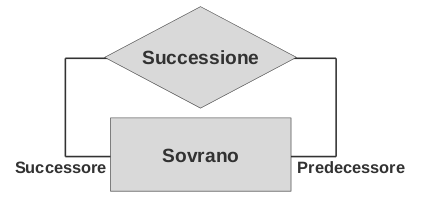
\includegraphics[scale=2.5]{img/bas8.png}
\end{center}
\newpage
\begin{esempio}
Descrivere lo schema concettuale della seguente
realtà:
Degli impiegati interessa il codice fiscale, il nome, il
cognome, i dipartimenti ai quali afferiscono (con la
data di afferenza), ed i progetti ai quali partecipano.
Dei progetti interessa il nome, il budget, e la città in
cui hanno luogo le corrispondenti attività. Alcuni
progetti sono parti di altri progetti, e sono detti loro
sottoprogetti. Dei dipartimenti interessa il nome, il
numero di telefono, gli impiegati che li dirigono, e la
città dove è localizzata la sede. Delle città interessa
il nome e la regione:
\begin{center}
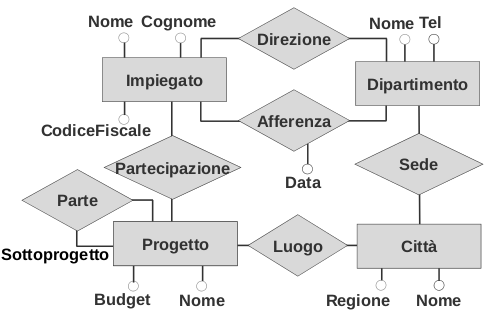
\includegraphics[scale=3]{img/er.png}
\end{center}
\end{esempio}
Si sceglie di modellare:
\begin{itemize}
\item un'\textbf{entità}:
\begin{itemize}
\item se le sue istanze sono concettualmente significative
indipendentemente da altre istanze
\item se ha o potrà avere delle proprietà indipendenti dagli
altri concetti
\item se il concetto è importante nell'applicazione
\end{itemize}

\item un \textbf{attributo}:
\begin{itemize}
\item se le sue istanze non sono concettualmente significative
\item se non ha senso considerare una sua istanza
indipendentemente da altre istanze
\item se serve solo a rappresentare una proprietà locale di
un altro concetto
\end{itemize}
\end{itemize}
Si sceglie di modellare:
\begin{itemize}
\item un'\textbf{entità}:
\begin{itemize}
\item se le sue istanze sono concettualmente significative
indipendentemente da altre istanze
\item se ha o potrà avere delle proprietà indipendenti dagli
altri concetti
\item se ha o potrà avere relazioni con altri concetti
\end{itemize}
\item una \textbf{relazione}:
\begin{itemize}
\item se le sue istanze non sono concettualmente
significative indipendentemente da altre istanze, cioè
se le sue istanze rappresentano n-ple di altre istanze
\item se non ha senso pensare alla partecipazione delle sue
istanze ad altre relazioni
\end{itemize}
\end{itemize}
per esempio:
\begin{center}
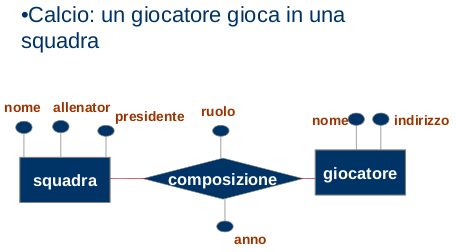
\includegraphics[scale=1]{img/er2.png}
\end{center}
qui ruolo è attributo della composizione perché un giocatore può cambiare ruolo e quindi ruolo non è attributo di giocatore.\\
\begin{esempio}
\begin{itemize}
\item ogni zoo è diviso in aree diverse a seconda che si tratti di rettili, pesci, uccelli, scimmie, grandi mammiferi, ... Ogni area è dotata di: nome,
indirizzo, dimensione, numero di sezioni.
\item per ogni tipo di animale ci sono informazioni che riguardano: classificazione zoologica, nome comune (giraffa, elefante, serpente,
tartaruga, ...), habitat, alimentazione, ... Per ogni tipo di animale c'è un diverso veterinario specialista, dipendente dello zoo.
\item ogni tipo di animale è rappresentato da esemplari e relativi dati anagrafici: nome proprio (giraffa Enrico, giraffa Giulia, ...), data di nascita,
Paese di provenienza, data di arrivo allo zoo, ...
\item ogni esemplare è dotato di più schede sanitarie contenenti ognuna: la data della visita, referto, dieta, nome del veterinario, ...

\end{itemize}
\begin{center}
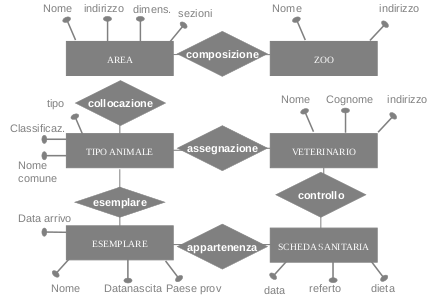
\includegraphics[scale=0.8]{img/er3.png}
\end{center}
lo zoo ha degli attributi che vanno indicati anche se non richiesti dalla traccia per evitare ambiguità. Dato che ogni scheda è collegata ad un veterinario, di cui ho un'entità la collego a veterinario con una relazione e non ne faccio  un attributo
\end{esempio}
Le relazioni possono avere una \textbf{cardinalità}, ovvero una coppia di valori che si associa a ogni entità
che partecipa a una relazione che specificano il numero minimo e massimo di
occorrenze delle relazione cui ciascuna
occorrenza di una entità può partecipare. Si rappresenta con un range tra un min e un max: $(min, max)$
\begin{center}
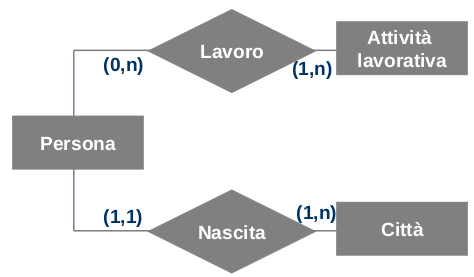
\includegraphics[scale=0.8]{img/er4.png}
\end{center}
Si hanno tre simboli:
\begin{enumerate}
\item 0 per la cardinalità minima indicante una \textit{partecipazione opzionale}
\item 1 per la cardinalità minima indicante una \textit{partecipazione obbligatoria} o indicante una cardinalità massima limitata
\item N indicante una cardinalità massima senza limite
\end{enumerate}
si hanno quindi relazioni:
\begin{itemize}
\item \textbf{uno a uno} se le cardinalità massime di
entrambe le entità sono uno, $(1,1)$ relazione $(1,1)$
\item \textbf{uno a molti}, $(0/1,1)$ relazione $(1,N)$
\item \textbf{molti a molti}, $(0/1,N)$ relazione $(0/1,N)$
\end{itemize}
\begin{center}
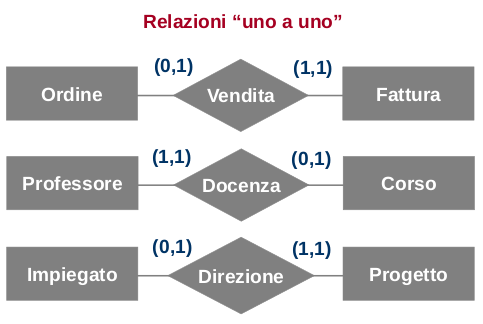
\includegraphics[scale=0.6]{img/er7.png}
\end{center}
\begin{center}
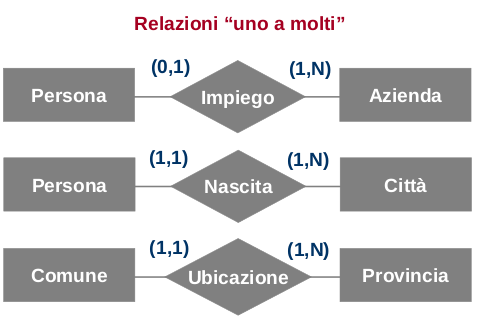
\includegraphics[scale=0.6]{img/er6.png}
\end{center}
\begin{center}
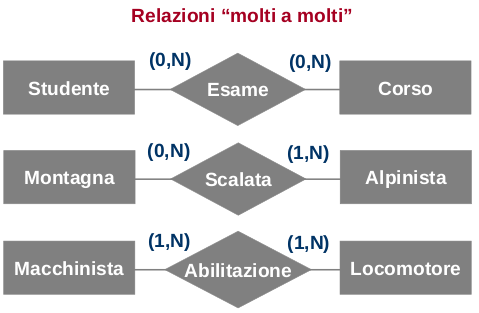
\includegraphics[scale=0.6]{img/er5.png}
\end{center}
\newpage
vediamo un esempio:
\begin{esempio}
si ha:
\begin{center}
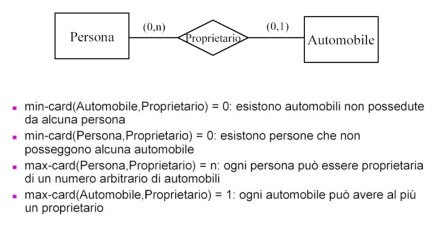
\includegraphics[scale=0.8]{img/er8.png}
\end{center}

\end{esempio}
Un vincolo di cardinalità tra una entita’ E e una relazione R
esprime un limite minimo (cardinalità minima) ed un limite
massimo (cardinalità massima) di istanze della relazione R a cui può partecipare ogni istanza dell'entità E.
Serve a caratterizzare meglio il significato di una relazione. La cardinalità minima deve essere minore di quella massima. Ovviamente si possono avere altri simboli:
\begin{center}
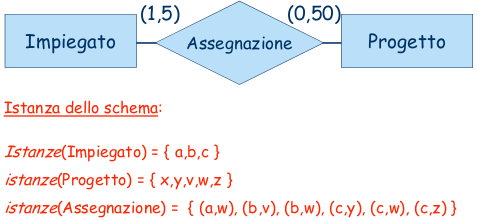
\includegraphics[scale=0.8]{img/er9.png}
\end{center}
\textit{Ad ogni impiegato sono assegnati da 1 a 5 progetti e ogni progetto è assegnato ad al più 50 impiegati. a,b,c compaiono in almeno una istanza di Assegnazione. x non compare nelle istanze di Assegnazione. Infine ci sono progetti (ad esempio lanciati da poco
tempo) che possono non essere assegnati a nessun
impiegato}\\
Si può mettere cardinalità agli attributi per indicare l'opzionalità o indicare attributi multivalore:
\begin{center}
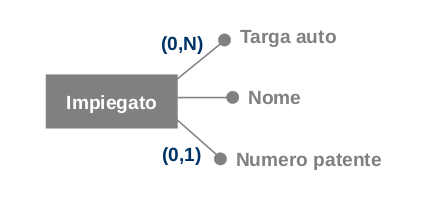
\includegraphics[scale=0.8]{img/er10.png}
\end{center}
\begin{center}
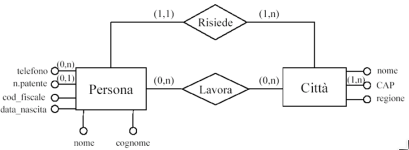
\includegraphics[scale=0.8]{img/er11.png}
\end{center}
infatti, per esempio, una persona può non avere la patente etc...\\
Un \textbf{identificatore di una entità} permette l'identificazione univoca delle occorrenze di un'entità. È formato da:
\begin{itemize}
\item attributi dell'entità, \textit{identificatore interno}, tipo il codice fiscale. Si ha la seguente notazione:
\begin{itemize}
\item se l'identificatore è formato da un solo attributo, si annerisce il corrispondente pallino
\item se l'identificatore è formato da più attributi, si uniscono gli attributi con una linea che termina con pallino annerito
\begin{center}
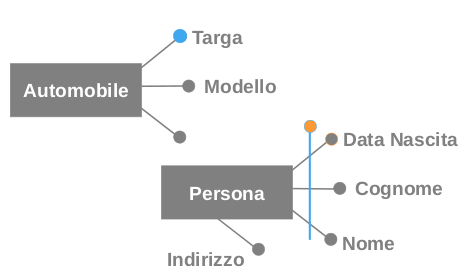
\includegraphics[scale=0.8]{img/er12.png}
\end{center}
\end{itemize}
\item (attributi +) entità esterne attraverso
relationship, \textit{identificatore esterno}, tipo la matricola che dipende dall'università. Come notazione si ha che l'identificatore è formato da attributi e relazioni (o meglio ruoli), si indica unendo gli attributi ed i ruoli con una linea che termina con pallino annerito:
\begin{center}
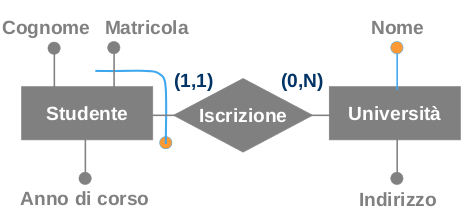
\includegraphics[scale=0.8]{img/er13.png}
\end{center}
\end{itemize}
Si hanno alcune osservazioni:
\begin{itemize}
\item ogni entità deve possedere almeno un
identificatore, ma può averne in generale più di uno
\item una identificazione esterna è possibile solo
attraverso una relationship a cui l'entità da
identificare partecipa con cardinalità $(1,1)$
\end{itemize}
vediamo un esempio complesso, che è preso da un vecchio esempio:
\begin{center}
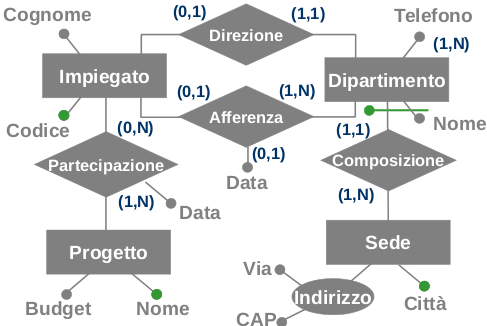
\includegraphics[scale=0.8]{img/er14.png}
\end{center}
\end{document}
